% \documentclass[10pt]{beamer}
\documentclass[xcolor=svgnames, t, aspectratio=169]{ctexbeamer}
\usepackage{booktabs}
\usepackage{makecell}

\usetheme[
%%% options passed to the outer theme
%    progressstyle=corner,   % either fixedCircCnt, movCircCnt, or corner
%    rotationcw,                 % change the rotation direction from counter-clockwise to clockwise
%    shownavsym                  % show the navigation symbols
  ]{tarusimple}

% 加载宏包
%===================注意======================%
% 在调用beamer.cls宏包后,以下宏包将自动调用,
% 不应单独调用这些宏包,以免发生冲突
% amsfonts, amsmath, amssymb, amsthm, 
% enumerate, geometry, graphics, graphicx, 
% hyperref, url, 
% ifpdf, keyval, xcolor, xxcolor
% =============================================%

% 加载需要的宏包
\usepackage{csquotes}

% 符号字体
\usepackage{fontawesome5}

\usepackage{comment}

%%% Local Variables: 
%%% mode: latex
%%% TeX-master: "../main.tex"
%%% End:


%% 自定义相关的名称宏命令
%% ==================================================
%% \newcommand{\yourcommand}[参数个数]{内容}
% 塔里木大学各单位名称
\newcommand{\taru}{塔里木大学}
\newcommand{\cie}{信息工程学院}
\newcommand{\ciee}{信息与电气工程学院}

%% 签署春秋学期日期命令
\newcommand{\tomonth}{
  \the\year 年\the\month 月
}


\newcommand{\tomonthen}{
  \ifcase\the\month
  \or January%
  \or February%
  \or March%
  \or April%
  \or May%
  \or June%
  \or July%
  \or August%
  \or September%
  \or October%
  \or November%
  \or December%
  \fi, \the\year
}

\newcommand{\tosemester}{
  \the\year 年\ 
  \ifcase\the\month
  \or 秋%
  \or 春%
  \or 春%
  \or 春%
  \or 春%
  \or 春%
  \or 春%
  \or 夏%
  \or 秋%
  \or 秋%
  \or 秋%
  \or 秋%
  \fi
}

\newcommand{\tosemesteren}{
  \ifcase\the\month
  \or Autumn%
  \or Spring%
  \or Spring%
  \or Spring%
  \or Spring%
  \or Spring%
  \or Summer%
  \or Autumn%
  \or Autumn%
  \or Autumn%
  \or Autumn%
  \or Autumn%
  \fi, \the\year
}

% 插图路径设置
% ==================================================
\graphicspath{{figs/}}%图片所在的目录
% ==================================================

% 为标题页/封底页指定一个 logo
\pgfdeclareimage[height=0.5cm]{titlepagelogo}{cauname}% 标题页
\titlegraphic{% 标题页底部
  \pgfuseimage{titlepagelogo}
}


% 载入需要的TiKZ库
\usetikzlibrary{chains}

%% 设置绘制目录结构的宏及参数
\usepackage[edges]{forest}
\definecolor{folderbg}{RGB}{124,166,198}
\definecolor{folderborder}{RGB}{110,144,169}
\newlength\Size
\setlength\Size{4pt}
\tikzset{%
  folder/.pic={%
      \filldraw [draw=folderborder, top color=folderbg!50, bottom color=folderbg] (-1.05*\Size,0.2\Size+5pt) rectangle ++(.75*\Size,-0.2\Size-5pt);
      \filldraw [draw=folderborder, top color=folderbg!50, bottom color=folderbg] (-1.15*\Size,-\Size) rectangle (1.15*\Size,\Size);
    },
  file/.pic={%
      \filldraw [draw=folderborder, top color=folderbg!5, bottom color=folderbg!10] (-\Size,.4*\Size+5pt) coordinate (a) |- (\Size,-1.2*\Size) coordinate (b) -- ++(0,1.6*\Size) coordinate (c) -- ++(-5pt,5pt) coordinate (d) -- cycle (d) |- (c) ;
    },
}
\forestset{%
declare autowrapped toks={pic me}{},
declare boolean register={pic root},
pic root=0,
pic dir tree/.style={%
for tree={%
    folder,
    %font=\ttfamily,
    grow'=0,
    s sep=1.0pt,
    font=\small \sffamily,
    %fit=band,
    %ysep = 1.0pt,
    inner ysep = 2.6pt,
  },
before typesetting nodes={%
for tree={%
edge label+/.option={pic me},
},
if pic root={
tikz+={
\pic at ([xshift=\Size].west) {folder};
},
align={l}
}{},
},
},
pic me set/.code n args=2{%
    \forestset{%
      #1/.style={%
          inner xsep=2\Size,
          pic me={pic {#2}},
        }
    }
  },
pic me set={directory}{folder},
pic me set={file}{file},  
}
%% ==================================================


%%% Local Variables: 
%%% mode: latex
%%% TeX-master: "../main.tex"
%%% End: 
  
  
\title{中国农业大学博士入学复试报告}
%\subtitle{基于冠层改进的Cotton2K模型}
\date[2022/4/24]{\zhdate{2022/4/24}}
\author[唐梓涯]
{唐梓涯}
\institute
{
  \ciee
  
}

\begin{document}

{\taruwavesbg%
\begin{frame}[plain,noframenumbering]
  \titlepage
\end{frame}
}

\begin{frame}{目录}{内容列表}
  \begin{enumerate}
    \item 个人基本情况
    \item 教育经历
    \item 工作经历
    \item 科研经历
    \item 取得成果
  \end{enumerate}
\end{frame}

\begin{frame}{个人基本情况}{}
  本人名叫唐梓涯,30 岁,江苏如东人,中共预备党员。
\end{frame}

\begin{frame}{教育经历}{毕业院校、专业}
  \begin{table}
    %\caption{本科、硕士就读院校及专业}
    \begin{tabular}{cc}
      本科                                       & 硕士                                                           \\
      
\includegraphics[scale=1.15]{ppcnwafu.png} & 
\includegraphics[scale=0.5,trim=88 71 66 77,clip]{cietaru.png} \\
      2010{-}2014                                & 2019至今\\
      植物保护 (090103)                          & 农业电气化与自动化 (082804)
    \end{tabular}
  \end{table}
\end{frame}
\begin{frame}{工作经历}{南京振古}
  \begin{center}
    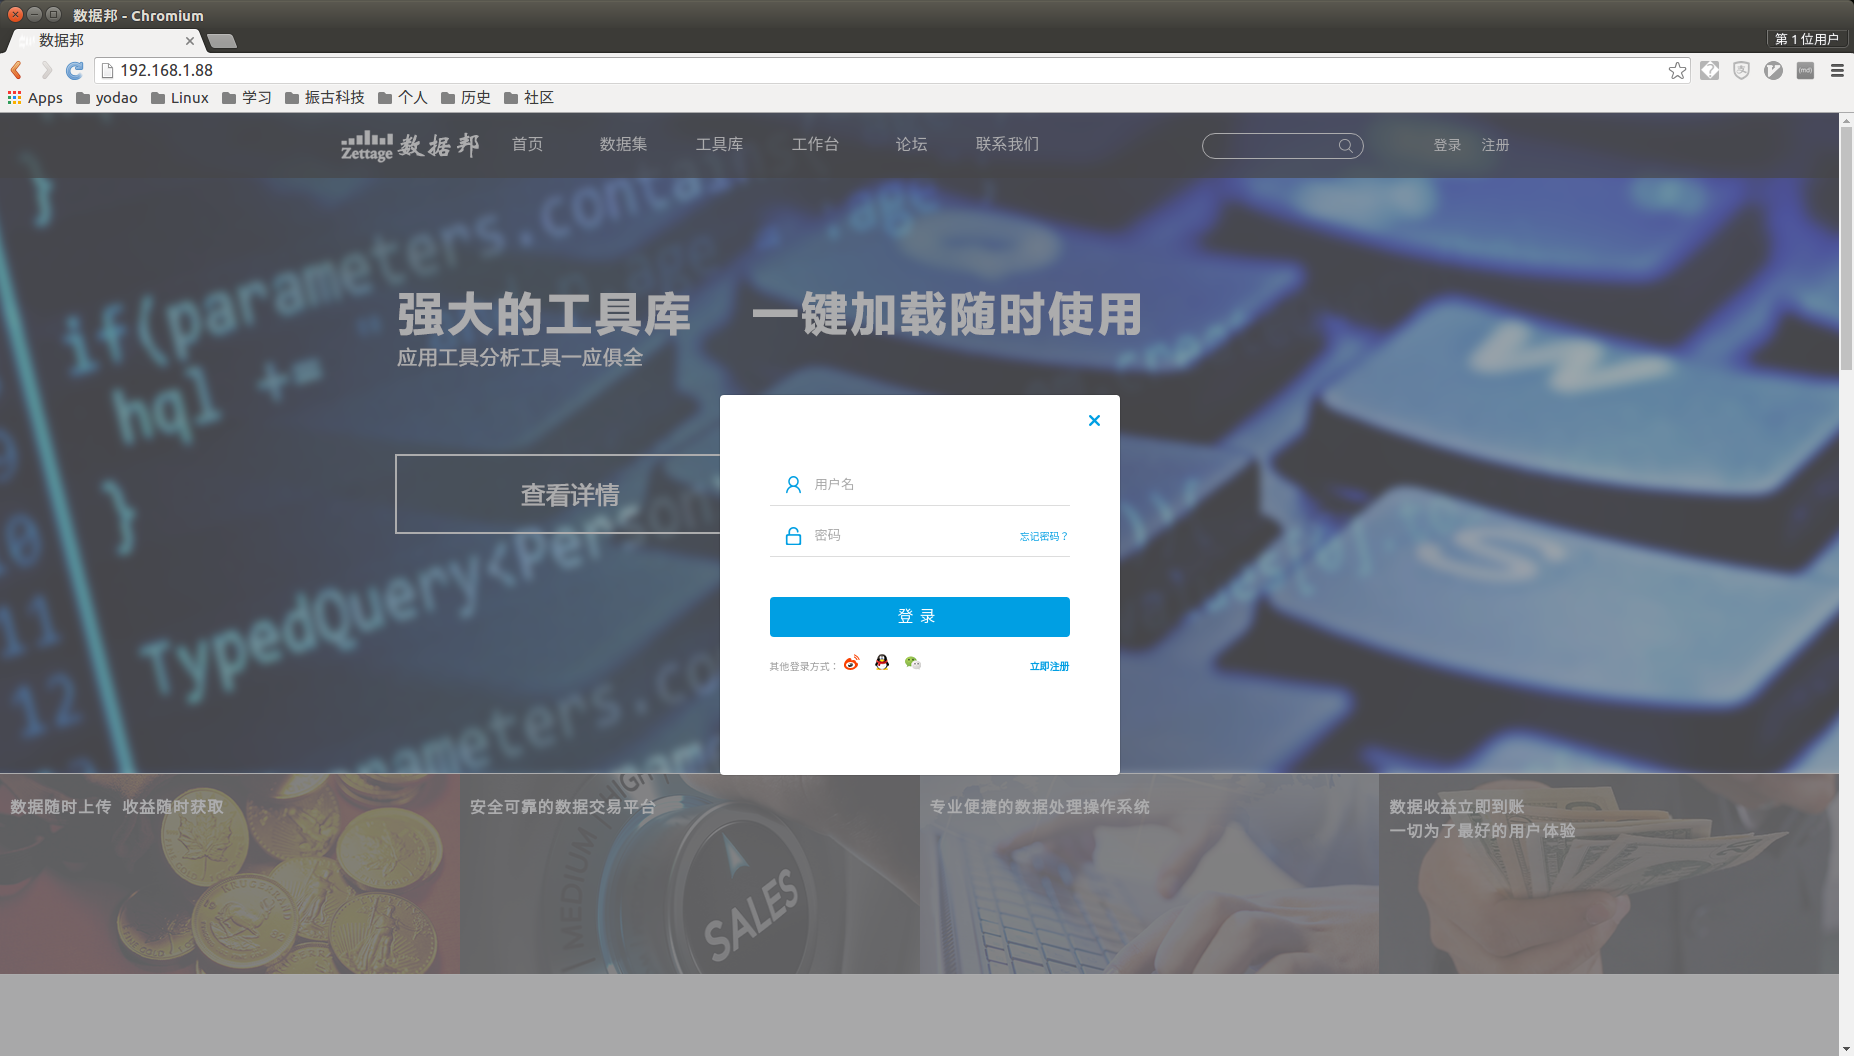
\includegraphics[scale=0.18]{zettage.png}
  \end{center}
\end{frame}
\begin{frame}{工作经历}{Microsoft}
  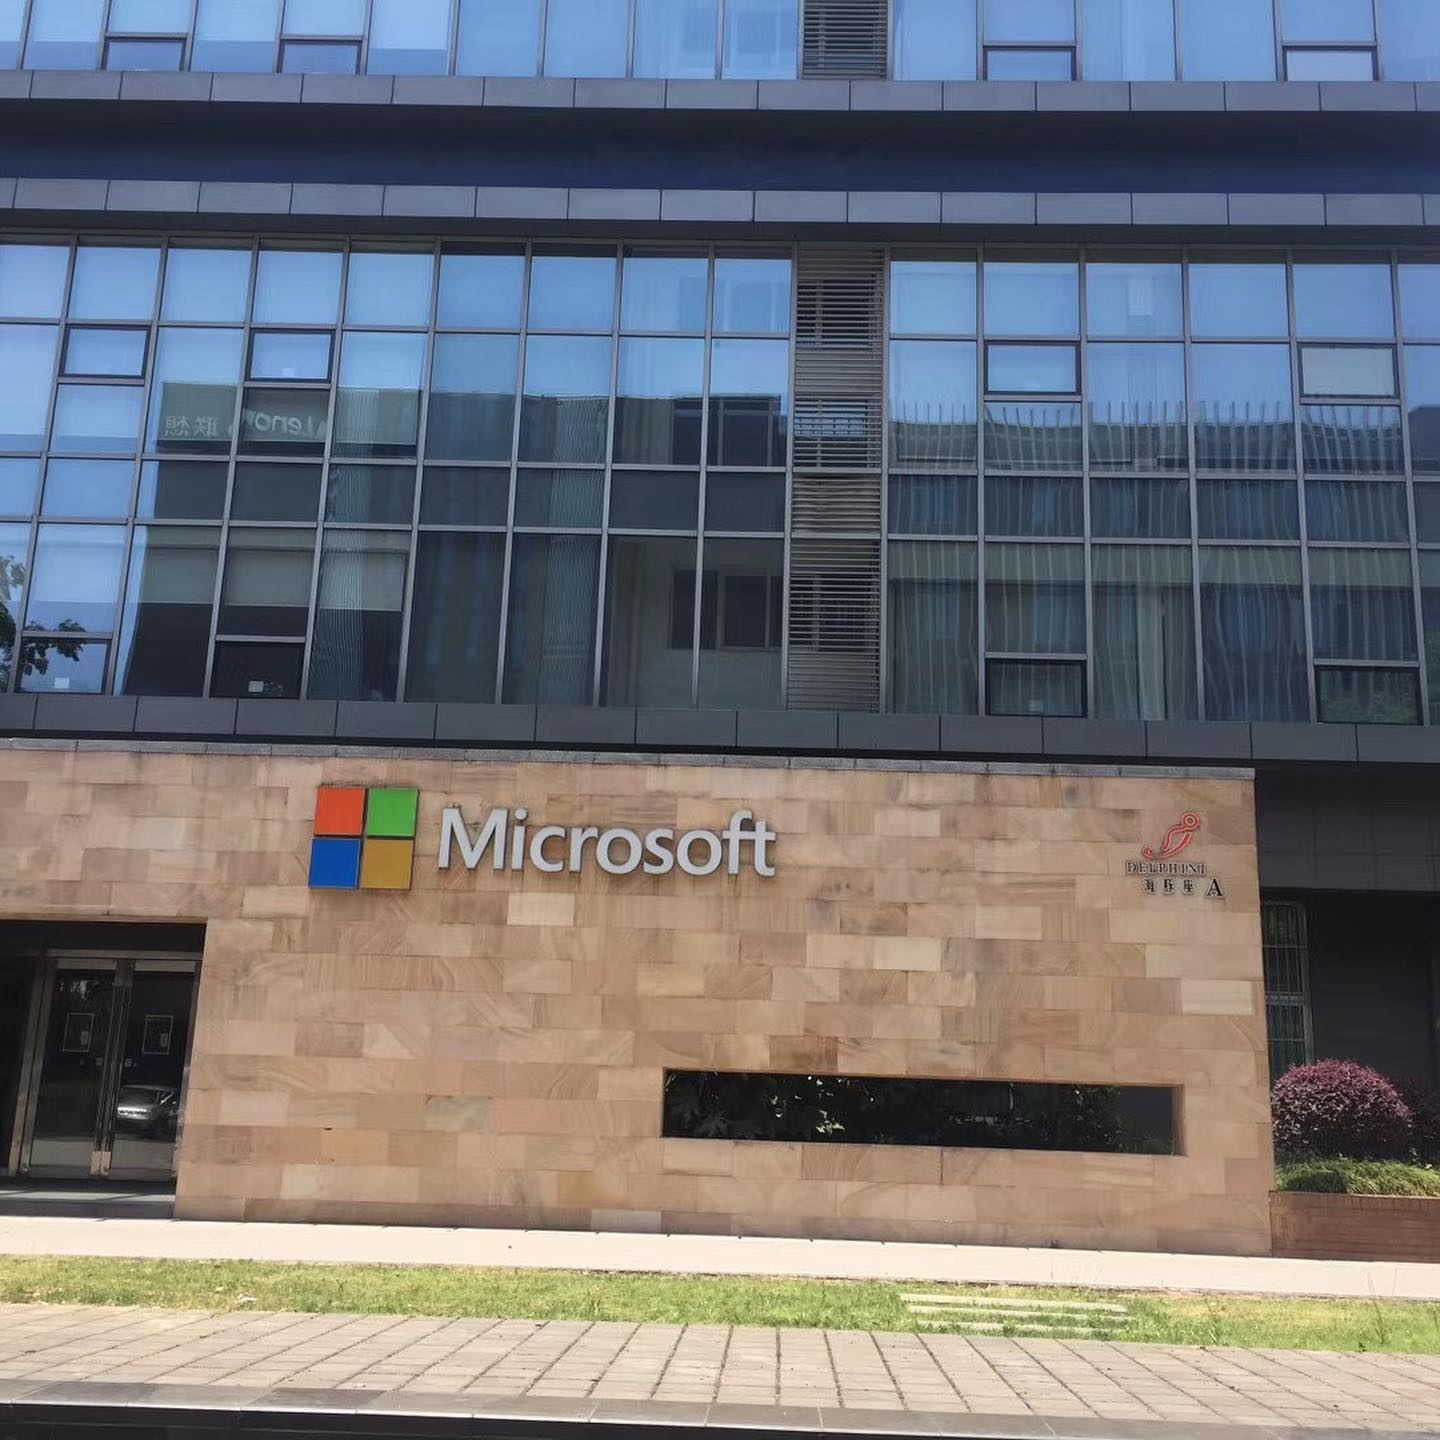
\includegraphics[scale=0.14,trim=0 0 0 120,clip]{microsoft_css.jpg}
  
\includegraphics[scale=0.2]{azure.png}
\end{frame}
\begin{frame}{工作经历}{科大讯飞}
  \begin{center}
    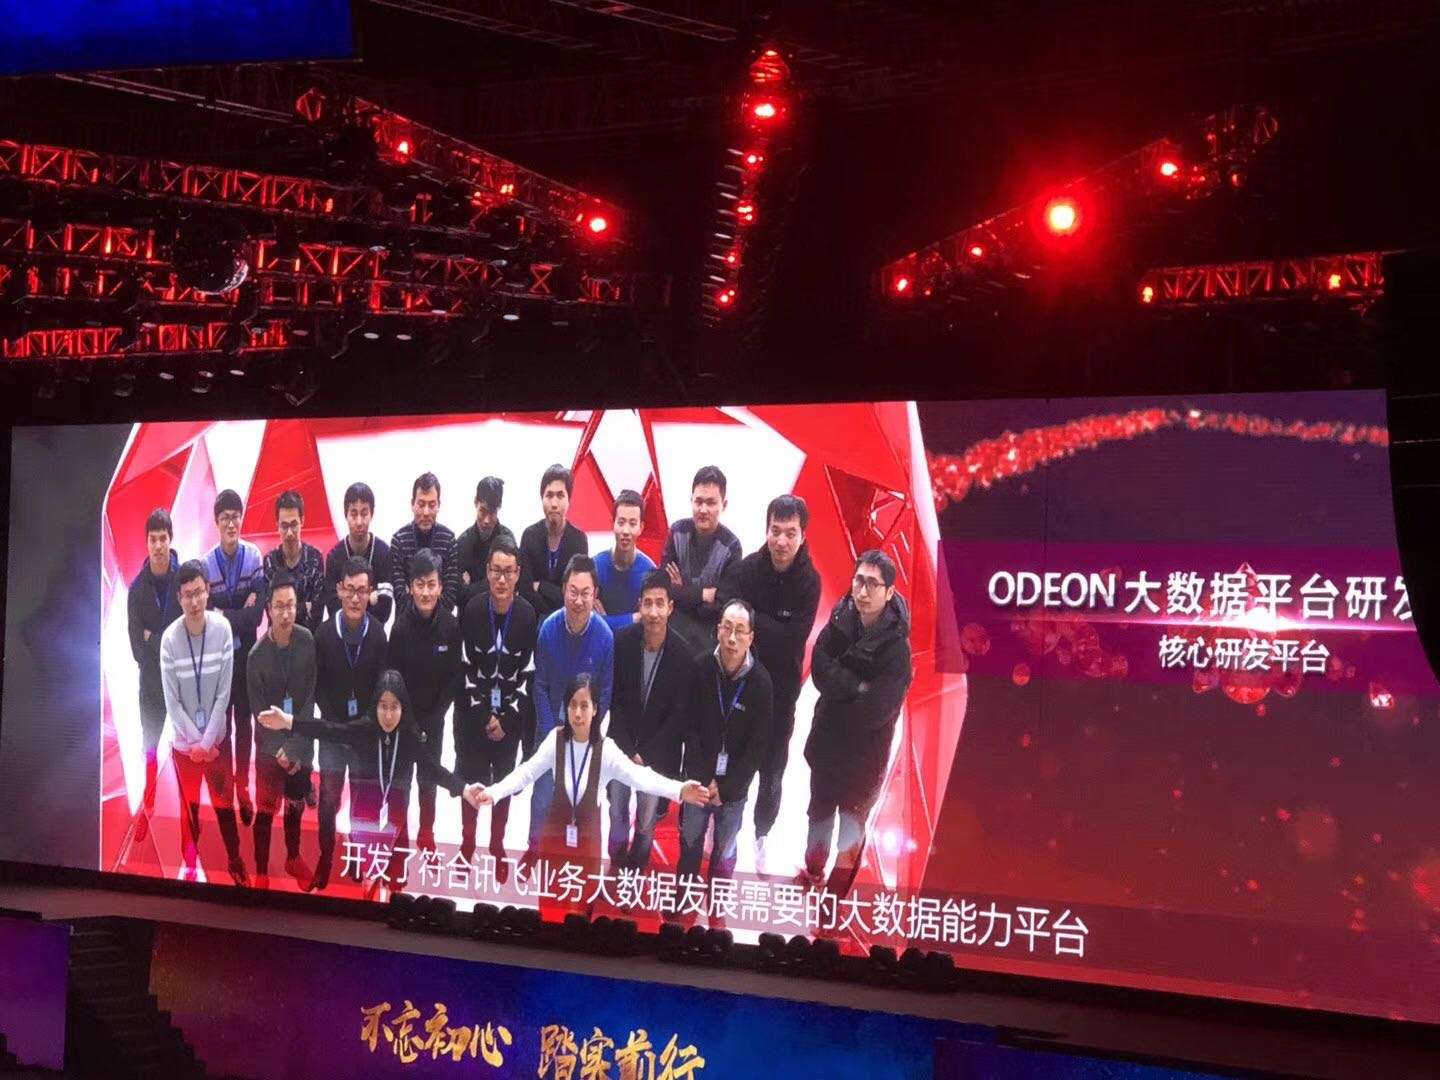
\includegraphics[scale=0.2,trim=0 0 0 300,clip]{iflytek.jpg}
  \end{center}
\end{frame}
\begin{frame}{科研经历}{维哈语料库}
  % \begin{center}
  %   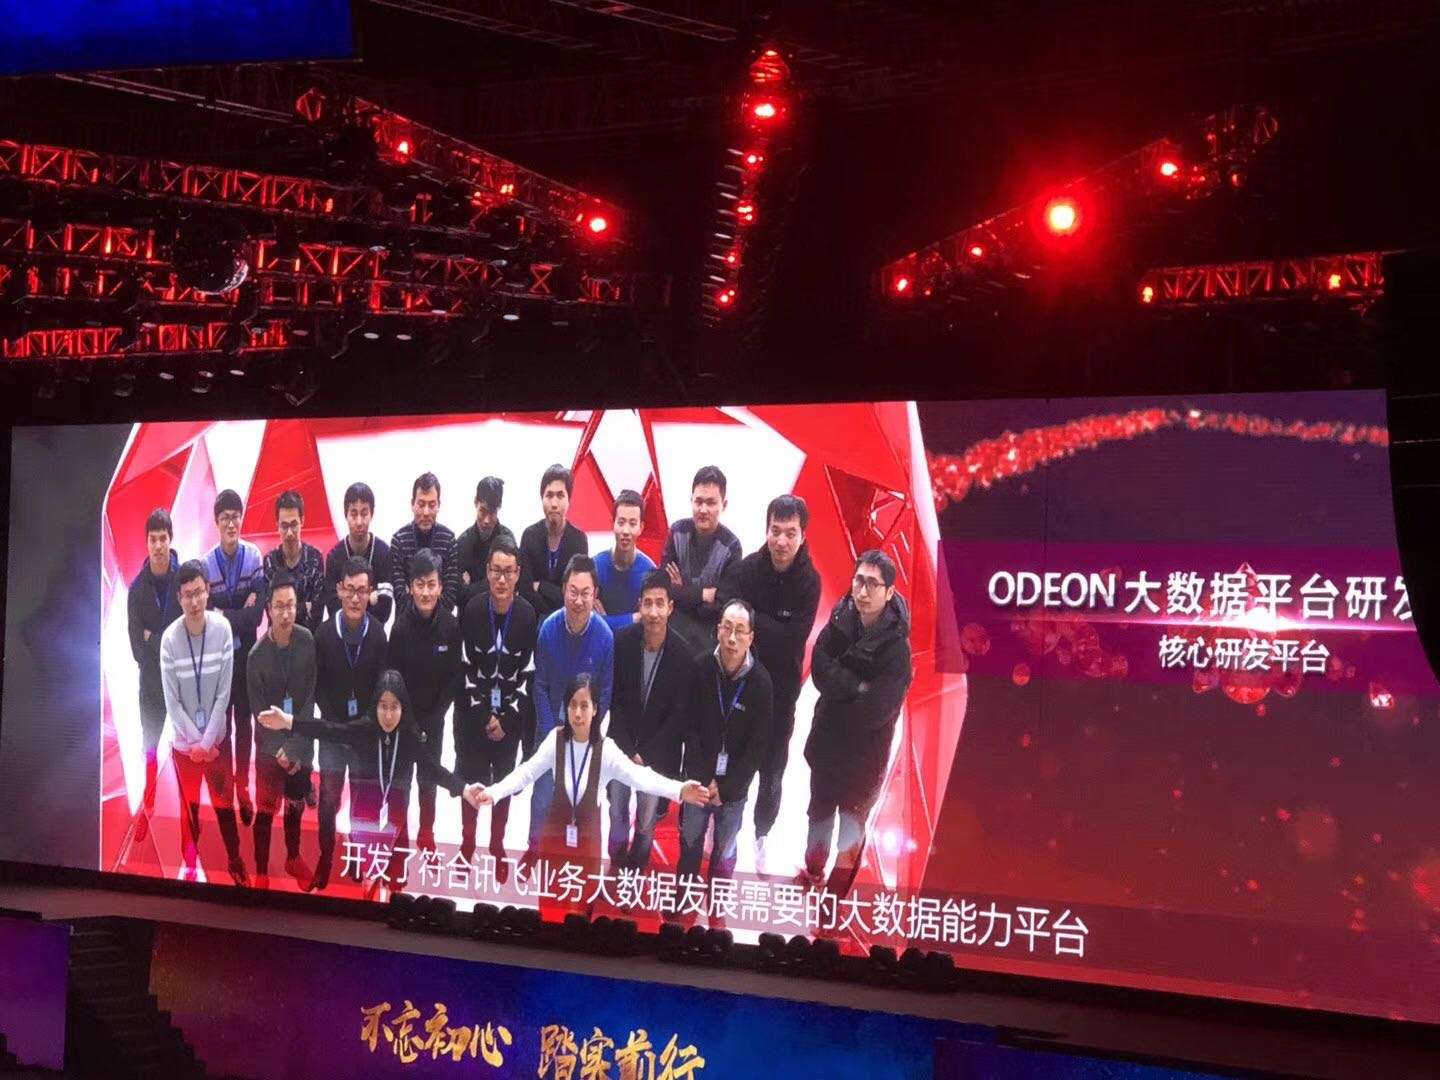
\includegraphics[scale=0.2,trim=0 0 0 300,clip]{iflytek.jpg}
  % \end{center}
\end{frame}
{\taruwavesbg
\begin{frame}[plain,noframenumbering]
  \finalpage{谢谢各位老师同学聆听!\\欢迎大家多提宝贵意见和建议!}
\end{frame}
}

\end{document}
